\documentclass{article}
\usepackage[fleqn]{amsmath}
\usepackage{graphicx}
\graphicspath{{Images/}}
\begin{document}
	\noindent Name : Febrian Nugroho\\
	NIM :2301930551
	\begin{center}
		\Large Answer of Assignment II\\
		\Large Adaptive Linear Neuron\\
	\end{center}
	\normalsize
	Dataset:
	\begin{enumerate}
		\item $\left\{x_1=\begin{bmatrix}
			-1 \\ 2
		\end{bmatrix}, t_1=1\right\}$
		\item $\left\{x_2=\begin{bmatrix}
			0 \\ 2
		\end{bmatrix}, t_2=1\right\}$
		\item $\left\{x_3=\begin{bmatrix}
			3 \\ -2
		\end{bmatrix}, t_3=1\right\}$
		\item $\left\{x_4=\begin{bmatrix}
			-2 \\ -1
		\end{bmatrix}, t_4=-1\right\}$
		\item $\left\{x_5=\begin{bmatrix}
			0 \\ -3
		\end{bmatrix}, t_5=-1\right\}$
	\end{enumerate}
	Initial Weight and Bias: \\
	w = $\begin{bmatrix}
		3.0 & 1.0
	\end{bmatrix}$ \\
	b = 1.0 \\
	$\alpha$ = 0.05 \\
	\begin{center}
		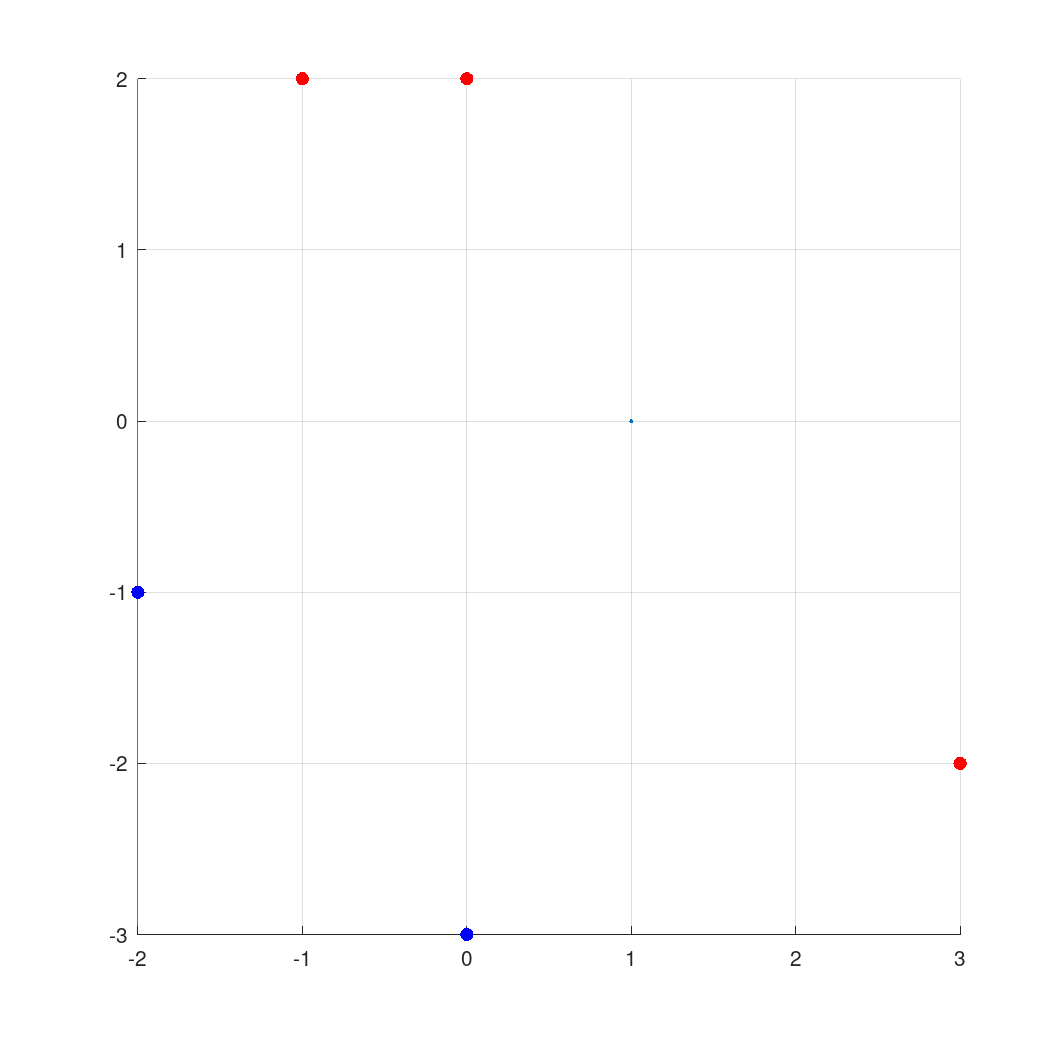
\includegraphics[width=0.7\textwidth]{initial_plot.png} \\
		\Large Algorithm
	\end{center}
	for each iteration, 
	\\ 1. calculate output:
	\begin{align*}
		a_j & = \sum w_{ij} p + b,~\text{where}\\
		a_j & = \text{Output}, w = \text{Weight}, p = \text{Input},~\text{and}~b = \text{Bias}
	\end{align*}
	\\ 2. compute loss function / error:
	\begin{align*}
		E(k) & = (t_k - a_k)^2,~\text{where} \\
		E(k) & = \text{Least Square Error}~, \\
		t_k & = \text{Desired target input}, \\
		a_k & = \text{Output}
	\end{align*}
	\\ 3. Update weights:
	\begin{align*}
		w_{new} & = w_{old} + \Delta w, ~\text{where} \\
	\end{align*}
	Training \\
	1th Iteration: \\
	\begin{equation}
	\begin{split}
		a_1 & = w.x+b \\
		& = \begin{bmatrix}
			3.0 & 1.0
		\end{bmatrix}. \begin{bmatrix}
		-1 \\ 2
	\end{bmatrix} + 10 \\
	a_1 & = 9
	\end{split}
	\end{equation}
	\begin{equation}
	\begin{split}
		w_{new} & = w_{old} + w_\Delta, dengan \\
		w_{\Delta} & = 2 \alpha e x \\, dan \\
		e & = t - a
	\end{split}
	\end{equation}
	\begin{equation}
	\begin{split}
		w_{new} & = w_{old} + (2 \alpha e x) \\
		w_{new} & = \begin{bmatrix}
			3.0 & 1.0
		\end{bmatrix} + (2 * 0.05 * )
	\end{split}
	\end{equation}
\end{document}
